%%% Magic comments for setting the correct parameters in compatible IDEs
% !TeX encoding = utf8
% !TeX program = pdflatex
% !TeX spellcheck = en_US

\documentclass[11pt,a4paper]{report}

\usepackage[margin=25mm]{geometry}
\usepackage[T1]{fontenc}
\usepackage{graphicx}
\usepackage{hyperref}
\usepackage{booktabs}
\usepackage{tabularx}

\newcolumntype{Y}{>{\raggedright\arraybackslash}X}

\hypersetup{
  colorlinks=true,
  linkcolor=blue,
  citecolor=blue,
  urlcolor=blue
}
\setlength{\parskip}{0.5em}
\setlength{\parindent}{0pt}
\setlength{\tabcolsep}{4pt}

%% Title page for the technical report
\begin{document}
\hypersetup{pageanchor=false}
\begin{titlepage}
  \thispagestyle{empty}
  \centering
  
\includegraphics[width=0.9\textwidth]{images/ELVIS.pdf}\\
  \vspace{2cm}
  {\LARGE Technical Report}\par
  {\LARGE \bfseries [Project name]}\\
  \vspace{1cm}
  {\large [Author name(s)]\\\mbox{[Group X]}}\\
  \vspace{1cm}
  \vfill
  {\large\textbf{Use the provided structure as a guide for documenting the completed 
  demonstrator. Adapt the level of detail to the project while ensuring that all 
  relevant assessment criteria are addressed.}\par}
  \vspace{1cm}
  \textbf{Written Technical Report (10\%)}\\
  Deliverable: PDF \quad Due: 4 December, 23:59\par
\end{titlepage}

%% Abstract
\pagenumbering{roman}
\hypersetup{pageanchor=true}
\chapter*{Abstract}

%% Edit the abstract here: summarize the demonstrator's purpose, sensors,
%% implementation, validation, and most important supported result.
[In a short paragraph, state the demonstrator's purpose, the sensors used,
the main implementation, how it was validated, and the most important result.
Do not claim results that are not supported by the tests below.]

%% Table of contents
\tableofcontents
\clearpage
\pagenumbering{arabic}

%% Import each chapter from its own file.
%% Set the project context, users, final requirements, and acceptance criteria.
\chapter{Introduction and final requirements}
\label{sec:introduction}

Describe the problem addressed, intended users, and the purpose of the
completed demonstrator. State the final requirements and measurable
acceptance criteria. Briefly describe significant changes from the original
requirements and explain the reasons for these changes.

\begin{table}[htbp]
  \centering
  \caption{Final requirements and acceptance criteria.}
  \label{tab:requirements}
  \begin{tabularx}{\linewidth}{lYYY}
    \toprule
    ID & Requirement & Acceptance criterion & Verification section \\
    \midrule
    R1 & [What the final system must do] &
    [Observable, measurable pass condition] & [Section] \\
    R2 & [Add rows as needed] &
    [Threshold / condition] & [Section] \\
    \bottomrule
  \end{tabularx}
\end{table}

%% Summarize sensor characteristics, selection rationale, limitations, and sources.
\chapter{Sensors and technical characteristics}
\label{sec:sensors}

For each selected sensor, describe its type, measured quantity, and relevant
technical characteristics, including measurement range, resolution, accuracy,
and electrical/interface specifications. Explain why the sensor was selected
for the demonstrator, considering its suitability for the intended application.
Discuss relevant operating conditions, limitations, and placement
considerations. Support technical specifications with appropriate datasheet
references.

\begin{table}[htbp]
  \centering
  \caption{Sensors used in the delivered prototype. Add or remove rows as
  appropriate.}
  \label{tab:sensors}
  \begin{tabularx}{\linewidth}{YYYYY}
    \toprule
    Sensor / type & Quantity and range & Interface / supply &
    Resolution / accuracy & Selection rationale \\
    \midrule
    \mbox{[Sensor 1]} & [Quantity, units, range] & [Protocol, voltage] &
    [Specs and source] & [Reason] \\
    \mbox{[Sensor 2]} & [As applicable] & [As applicable] &
    [As applicable] & [As applicable] \\
    \bottomrule
  \end{tabularx}
\end{table}

%% Document the final system design, implementation, and operation.
\chapter{Implemented prototype}
\label{sec:prototype}

%% Show the system components, connections, interfaces, and data flow.
\section{System architecture}

Describe the implemented hardware and software architecture, interfaces,
power paths, and data flow. Include component names and versions where
relevant, and explain how the sensors, PSOC, user interface, and feedback
elements connect. Include a wiring diagram or electrical schematic showing
the relevant connections, pin assignments, and supply voltages.

\begin{figure}[htbp]
  \centering
  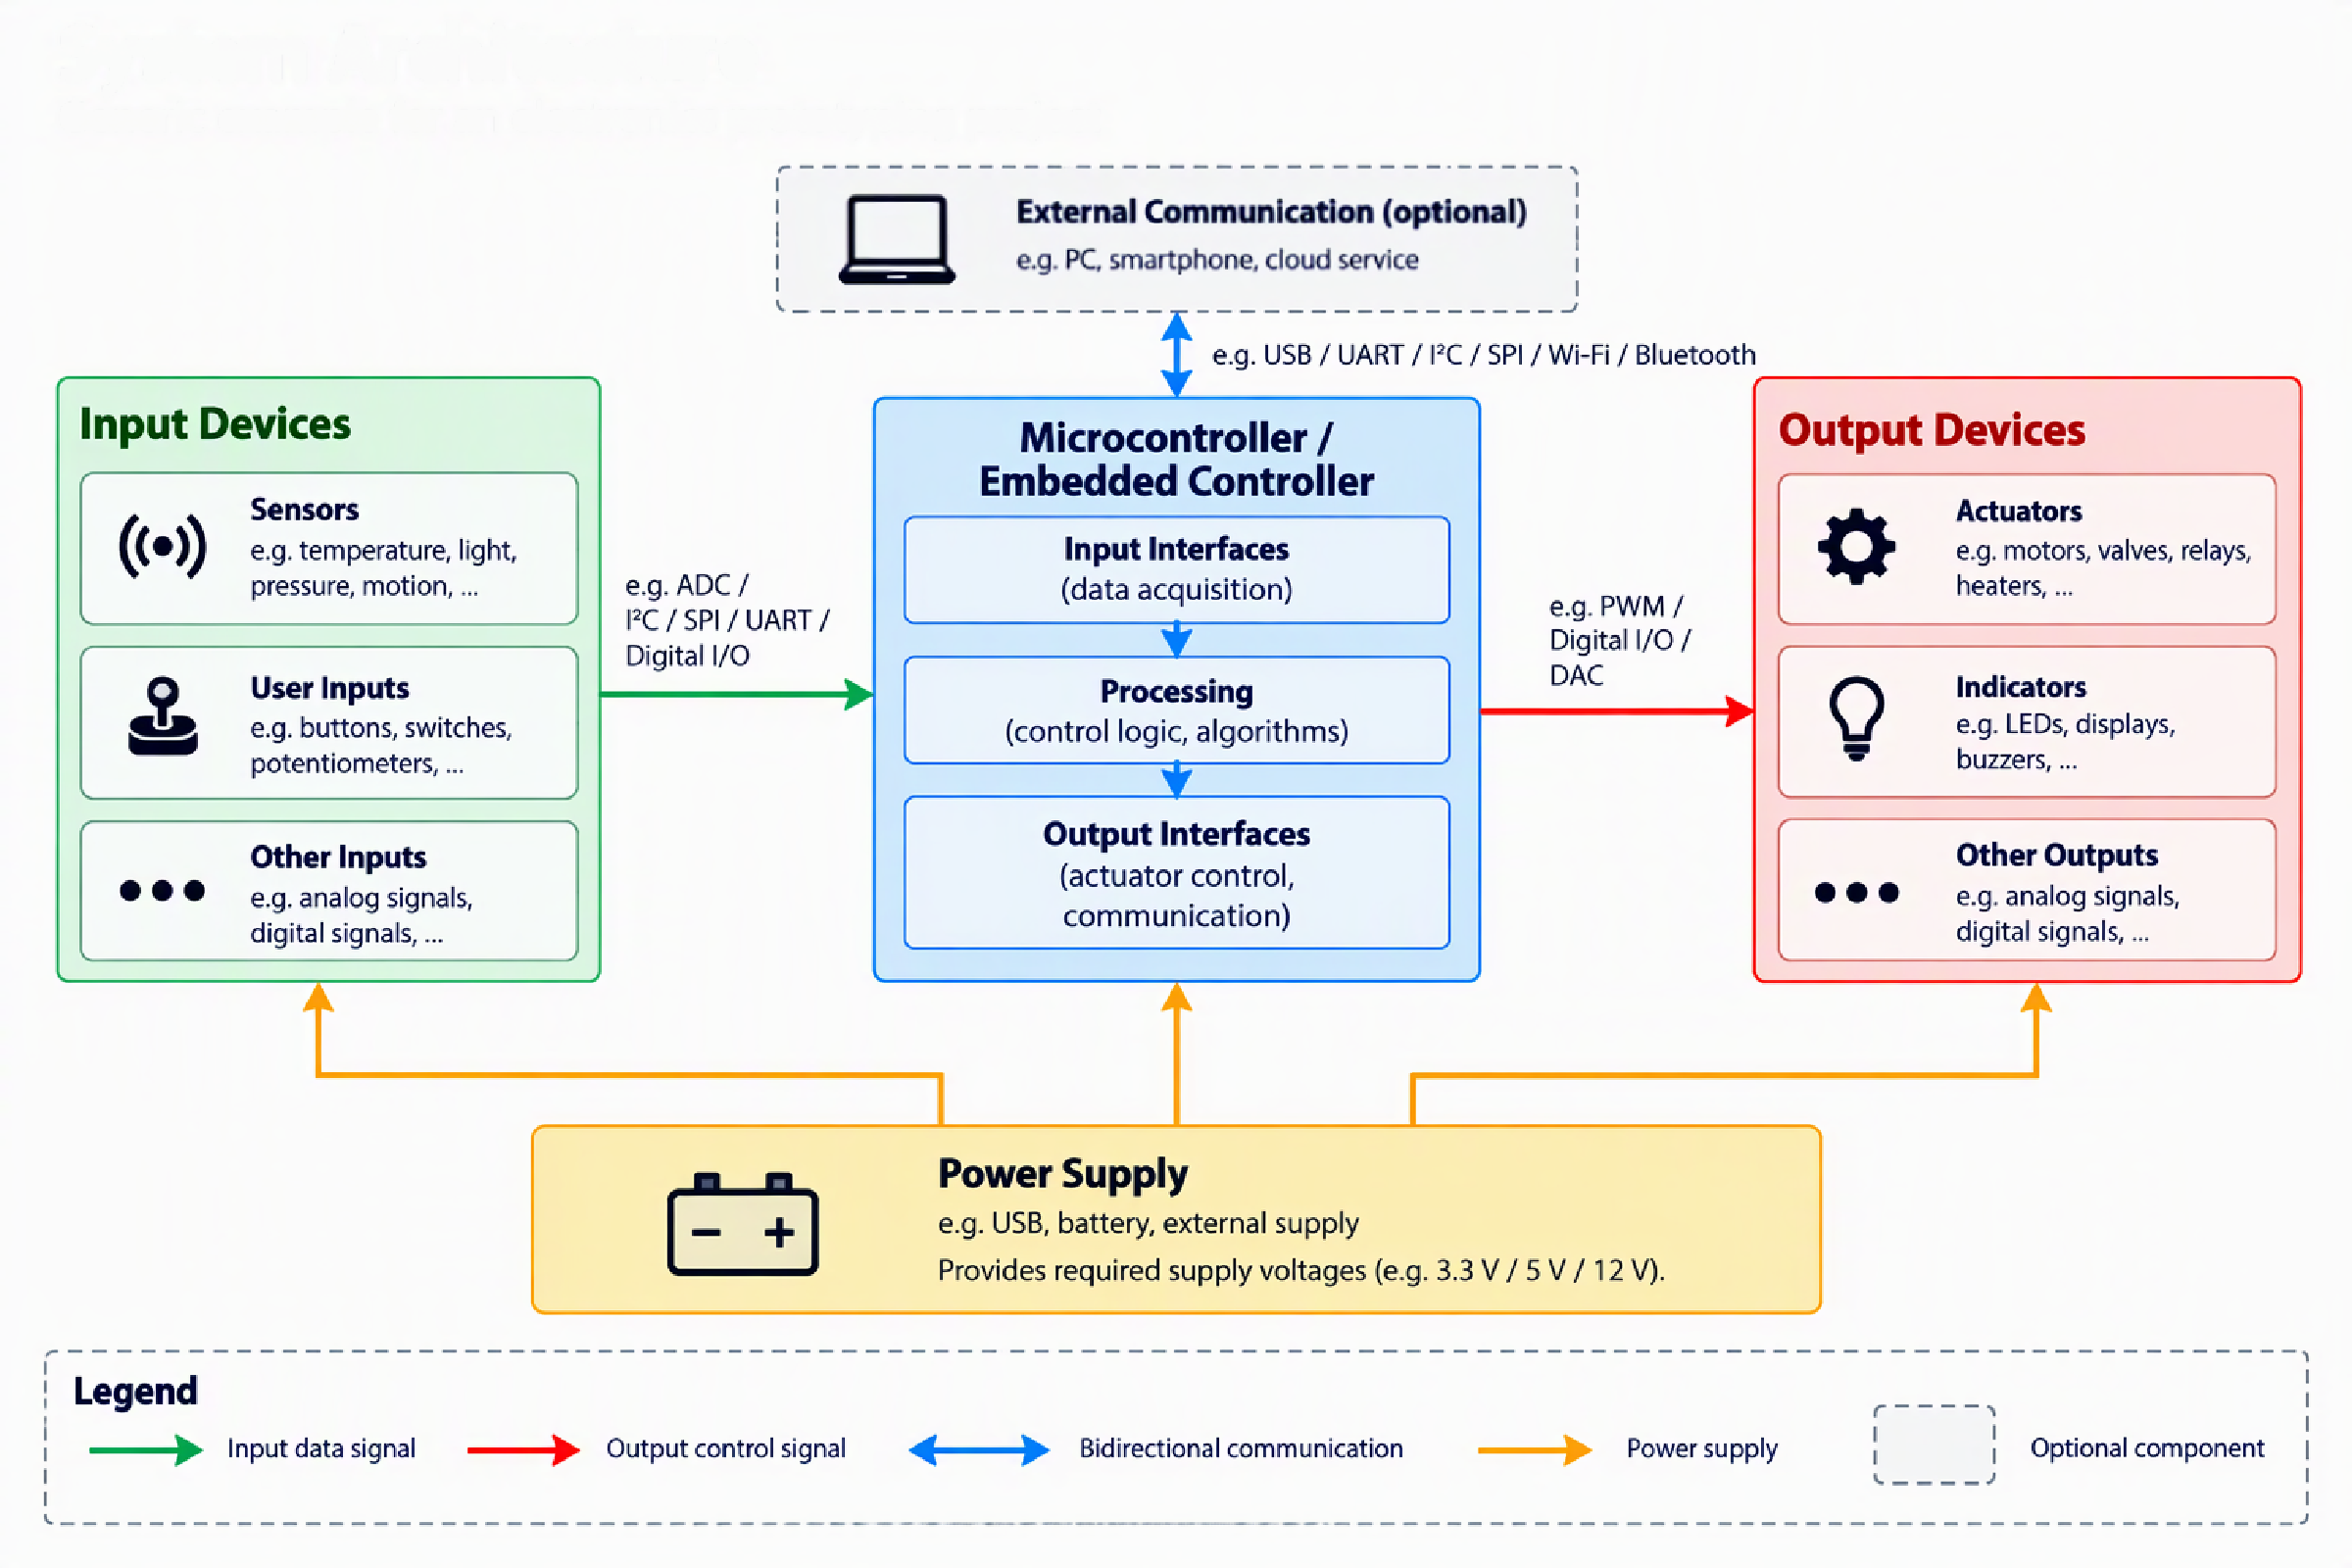
\includegraphics[width=0.9\linewidth]{images/system-architecture.pdf}
  \caption{Example system architecture diagram. Replace with a diagram of 
  the implemented demonstrator, showing the relevant components, interfaces, 
  and direction of data and control flow.}
  \label{fig:architecture}
\end{figure}

% Explain sensor acquisition, signal processing, scaling, and invalid readings.
\section{PSOC acquisition and processing}

Document the PSOC device and any external processing devices, including their
roles and relevant configuration. Describe sensor sampling frequency, signal
conditioning, conversion, filtering or other processing, units and scaling,
timing, and how invalid, missing, or out-of-range readings are handled.
Describe the path from the physical measurement to the displayed or otherwise
used value. Give enough detail to reproduce the configured behavior without
reproducing the entire source code.

% Describe how users operate the demonstrator and receive system feedback.
\section{Interaction and feedback}

Explain how a user operates the demonstrator, what information is presented,
and how the system provides feedback (for example, visual, audible, or
haptic). State how the user can interpret the readings and any status or
error indications. Include photographs of the completed demonstrator showing
its physical construction, sensor placement, and relevant user-interface
elements. Describe relevant interface design decisions and, if a
user-understanding evaluation was conducted, discuss its results in
Chapter~\ref{sec:results}.

% Record implementation details and the calibration method or its absence.
\section{Implementation and calibration}

Summarize the final implementation, including firmware/software versions,
important configuration, assembly, and any dependencies. Describe the
physical construction, mounting arrangements, and relevant mechanical
components. Include CAD models or manufacturing details where necessary to
understand or reproduce the implementation. Describe any calibration or
adjustment procedures performed, including the methods, reference equipment,
and relevant parameters. If no calibration was performed, state this
explicitly and discuss any implications for measurement accuracy.

% Identify relevant hazards, safeguards, limits, and operating precautions.
\section{Safety}

Identify relevant electrical, physical, environmental, and user risks.
Describe implemented safeguards, operating limits, and any precautions
required during setup and testing. Do not imply certification or safety
validation beyond the evidence available.

%% Define repeatable tests, conditions, equipment, and pass/fail criteria.
\chapter{Validation methods}
\label{sec:testing}

Select validation methods appropriate to the implemented functionality,
available equipment, and project requirements. Describe tests performed on
the final, completed prototype. For each test, describe its purpose, setup,
procedure, data recorded, and objective pass/fail criterion. Where relevant,
document the equipment, test conditions, repeated measurements, and
measurement uncertainty. Provide sufficient detail for the test to be
reproduced. Report deviations from the planned procedure.

% Describe tests of sensor performance against references or specifications.
\section{Sensor-characteristic tests}

Describe how relevant sensor characteristics or performance were evaluated,
such as measurement accuracy, repeatability, response time, detection
reliability, or recognition performance. Explain the test conditions,
methods, and reference measurements where applicable. Distinguish measured
performance from manufacturer specifications and acknowledge characteristics
that could not be verified.

% Describe tests of system functions, required conditions, and error handling.
\section{Demonstrator-function tests}

List the procedures used to verify acquisition, processing, display or other
outputs, feedback, error handling, and operation across the required
conditions. Where applicable, evaluate startup behavior, repeated operation,
and stability over time to identify intermittent failures or inconsistent
behavior. Link each procedure to requirement IDs in
Table~\ref{tab:requirements}.

% Explain how user understanding is evaluated and how responses are recorded.
\section{User-understanding evaluation (optional)}

If a user-understanding evaluation was conducted, describe the participants
in aggregate without identifying them, the tasks or questions given, the test
environment, how responses were recorded, and the criteria for judging
understanding. Address any relevant consent, privacy, or ethical considerations.
%% Present measurements and evaluate them against criteria and specifications.
\chapter{Results and analysis}
\label{sec:results}

Present measured results with units, sample counts, and uncertainty or
variation where appropriate. Use tables or figures where they make the
evidence clearer. Interpret results against both the acceptance criteria and
the relevant sensor specifications. Include failures and unexpected results;
do not report only successful trials.

\begin{table}[htbp]
  \centering
  \caption{Summary of final validation results.}
  \label{tab:results}
  \begin{tabularx}{\linewidth}{lYYYY}
    \toprule
    Test / req. & Procedure or condition & Result (with units) &
    Criterion & Outcome \\
    \midrule
    \mbox{[T1 / R1]} & [Brief test description] &
    [Observed result] & [Pass condition] & [Pass/fail] \\
    \mbox{[T2 / R2]} & [Add rows as needed] &
    [Observed result] & [Pass condition] & [Pass/fail] \\
    \bottomrule
  \end{tabularx}
\end{table}

Discuss what the evidence means for system performance and, where evaluated,
user understanding.
Explain any discrepancies, likely sources of error, and whether each
requirement was met, partly met, not met, or not tested. Point to the
supporting procedures and results.

%% Separate confirmed limitations from suspected issues and prioritize improvements.
\chapter{Limitations and future improvements}
\label{sec:limitations}

State limitations of the sensors, implementation, calibration, test methods,
sample size, operating conditions, and evidence. Identify unresolved issues
and distinguish confirmed limitations from suspected ones. Recommend
improvements that follow from the findings, prioritizing those that would
most improve reliability, safety, usability, or validation confidence.

%% Summarize the delivered system and evidence-supported conclusions.
\chapter{Conclusion}
\label{sec:conclusion}

Summarize what was built, the most important final test findings, and the
extent to which the final requirements were satisfied. Keep conclusions
proportional to the evidence; do not introduce new results here.

%% List the code, designs, test data, and setup details needed to reproduce the work.
\chapter*{Reproducibility materials}

List where a reader can obtain the firmware/source code, wiring or design
files, test data, and any additional setup instructions. Include version,
commit, or archive identifiers where available. If materials cannot be
shared, state why and provide the information needed to repeat the work
within that constraint.


%% Bibliography stays in the main report file.
\begin{thebibliography}{9}
  \bibitem{sensor-datasheet}
  [Manufacturer, ``Sensor datasheet title,'' document number and revision,
  publication date. URL and access date if online.]

  \bibitem{psoc-documentation}
  [Author or manufacturer, ``PSOC/device or development documentation,''
  version or revision, publication date. URL and access date if online.]

  \bibitem{other-reference}
  [Add references for methods, standards, or technical claims cited in the
  report. Use a consistent citation style.]
\end{thebibliography}

\end{document}
